\documentclass[12pt,man,draftfirst]{apa6}
\usepackage[nodoi]{apacite}
\bibliographystyle{apacite}
\usepackage{geometry} % see geometry.pdf on how to lay out the page. There's lots.
\usepackage{amsmath}
% \geometry{a4paper} % or letter or a5paper or ... etc
% \geometry{landscape} % rotated page geometry

% See the ``Article customise'' template for come common customisations

\title{Taking distributed representations seriously}
\shorttitle{Taking distributed representations seriously}
\author{Christopher R. Cox\\Timothy T. Rogers}
\affiliation{University of Wisconsin, Madison}

% \date{} % delete this line to display the current date
\abstract{The Parallel Distributed Processing (PDP) approach to cognition assumes that active mental representations are distributed over many neural populations. It is known that distributed representations can be acquired through domain general learning mechanisms to economically encode graded similarity structure that supports generalization and is robust to disruption. Until recently, however, the PDP hypothesis has not strongly influenced functional  brain imaging, which has, for historical and methodological reasons, tended to adopt modular 
assumptions about how the brain encodes information. Multivoxel pattern analysis (MVPA) relaxes these assumptions, but the most common methods are only sensitive to quite localized similarity structure, either within a searchlight or predetermined regions of interest. In this paper we leverage a recent innovation in multivariate analysis, the ``sparse overlapping sets Lasso'' (SOSLasso), to seriously consider whether distributed representations like those that arise in PDP models are also employed in the brain.By applying SOSLasso and univariate methods to data generated by artificial neural networks where the representational structure is known, we show how and why reliable univariate results can systematically miss important distributed patterns where SOSLasso preferentially identifies such patterns. We then apply both methods to real brain imaging data, and show that, at least in some domains of interest, the underlying representations appear to be distributed in ways that are highly consistent with the assumptions adopted by the PDP framework.}

\keywords{distributed representations, PDP, MVPA, SOSLasso, fMRI, cognitive neuroscience}

%%% BEGIN DOCUMENT
\begin{document}

\maketitle
% \tableofcontents

% INTRODUCTION
An important question for cognitive science concerns the nature of mental representations. What are they, how are they structured, where do they come from, and how do cognitive processes operate on them to support behavior? One approach to cognition, variously referred to as the parallel distributed processing (PDP), connectionist, or neural network approach, has offered fairly specific answers to these questions. It begins with the central tenet of cognitive neuroscience that all cognitive processes ultimately arise from the propagation of activity amongst large populations of neurons communicating their states via excitatory and inhibitory synaptic connections; but it further proposes that the important characteristics of such systems can be captured in simplified abstract form by computer models that simulate the flow of information through networks of neuron-like processing units connected by weighted synapse-like connections. All cognitive abilities are proposed to arise from representational and processing mechanisms that can be so described and understood. Accordingly, the framework offers a constrained view of what mental representations are: patterns of neural activity evoked by a stimulus or a process over a set of units operating in parallel. Often such representations are proposed to be highly distributed, so that (1) any given unit contributes to the representation of many different items, (2) any given item representation is encoded over many different units and (3) the representation inheres in the full pattern of activation over all units, and not in the activation of individual units.

The case for distributed representations runs much deeper than being an implementational detail within a particular modeling formalism. Indeed, distributed representations of this kind have several properties that make them useful for understanding various aspects of cognition. For instance, they provide a natural basis for similarity-based generalization \cite{greer_emergence_2001}. Two different items that generate overlapping patterns of activation over the same units will tend to produce similar responses downstream in the network. Thus distributed representations explain how prior learning supports the processing of novel inputs, an ability central to accounts of categorization, inductive inference, language processing, and many other cognitive phenomena. Similarity-based generalization also naturally produces patterns of behavior observed in many different tasks, such as typicality effects, frequency effects, and effects of quasi-regularity \cite{plaut_understanding_1996-1, rogers_object_2003}. Distributed representations explain why, with neuropathology, cognitive abilities are not disrupted in an all-or-none fashion, but instead degrade gracefully: when some units in the representation are destroyed or disrupted, the remaining units continue to communicate with downstream units, transmitting information that may still be at least approximately correct \cite{devlin_category-specific_1998,rogers_structure_2004}. They provide a means of understanding the acquisition of new representations: rather than adding new information to a database, or new representational elements into a processing system, new representations can be acquired by adjusting connections within the network so that a given stimulus or process generates a new pattern of activity over the existing units. Finally, distributed representations can be highly efficient. With a local code, in which each unit represents one and only one item of information, then with n units it is possible to represent just n items. With a binary distributed coded, the same n units can represent 2n distinct items; and if the units encode continuous activation values there is, in principle, no limit to the number of items a given set of units can encode \cite{hinton_distributed_1984}.

These virtues are well known and form the basis for influential accounts of healthy, disordered, and developing cognition in theories of reading \cite{patterson_connections_1989, seidenberg_distributed_1989}, inflectional morphology \cite{bird_deficits_2003, patterson_deficits_2001, plunkett_connectionist_1999}, semantic processing \cite{hoffman_semantic_2011,lambon_ralph_neural_2007,rogers_semantic_2004}, and many other domains. Perhaps surprisingly, however, remarkably little work in cognitive neuroscience has attempted to directly test PDP's assumptions about the nature of mental representations. The reasons for this gap are probably methodological, at least in part. The most ubiquitous methods in human cognitive neuroscience---fMRI and other functional brain imaging technologies---typically yield vast amounts of noisy data.  To discern interesting patterns in these datasets, or to test particular hypotheses, the statistical models employed must adopt specific assumptions about the nature of the underlying signal. For many years, standard statistical approaches were built upon representational assumptions that were at odds with those adopted under the PDP approach. As a result it has been difficult to relate the results of such analyses to the predictions of PDP models. This has begun to change with the advent of new multivariate methods for analyzing brain imaging data but many challenges still remain. Several different approaches have appeared in the literature in recent years, each carrying with it particular assumptions about the nature of the underlying neural code, and so bringing biases in the kind of signal it is capable of detecting. Moreover, the nature of the assumptions and their implications may not always be completely transparent. Thus, although the PDP framework (and related approaches) put forward quite specific hypotheses about the nature of representations in the mind and brain, it has not been clear how neuroscience methods, and in particular functional brain imaging, might best be leveraged to test these hypotheses.

The goal of the current paper is to consider how the analysis of brain imaging data might best be approached if the PDP assumptions about mental representation are valid. We first consider in more detail what the PDP assumptions are and why they pose challenges for standard and even many state of the art brain imaging methods. To illustrate these points, we compare and contrast the results yielded by five different statistical methods in the analysis of the activation patterns generated by different inputs to a simple PDP model. We take the activation of a single unit as a model analog of the mean activity in a population of neighboring neurons, similar to that estimated from changes in the BOLD response at a single voxel. Since the behavior, architecture, and representational structure embedded in the simple model are fully known, it is possible to measure the extent to which the various methods succeed in identifying the model components that encode interesting representational structure. This analysis thus illustrates the strengths and weaknesses of different approaches if PDP assumptions about representation are valid. The results suggest a new strategy for the analysis of functional imaging data that may help to better connect PDP models to cognitive neuroscience. We then assess the utility of this approach by comparing its results to those of other state of the art methods in the analysis of one well-known publicly released fMRI dataset.

\section{A brief overview of PDP models and the representational assumptions they adopt}
PDP models are composed of simple neuron-like processing units that communicate via weighted synapse-like connections. Each unit adopts an activation state, typically varying between 0 and 1, that can be viewed as expressing the mean firing rate of a population of spiking neurons proportional to their maximal rate. Units transmit information about their current activation through weighted connections, which can be viewed as capturing the net effect of activity in one population of neurons on another. Weights are typically real-valued, with negative numbers indicating a net inhibitory effect and positive numbers indicating a net excitatory effect. Each unit computes a simple process: it adjusts its current activation state according to the input it receives from other units in the networks. If a given receiving unit receives inputs from a set of n sending units, then the input is usually computed as the inner product of the activation across all sending units and the values of the weights projecting from the sending units to the receiving units. The unit then converts the net input into a new activation state according to a specified transfer function (often a sigmoidal function of the net input). All units are conceived as computing inputs and updating activation states in parallel (hence ``parallel'' distributed processing), though on serial computers this parallel process is simulated by updating units in randomly permuted order.

Within a network, units are generally organized into layers, which govern the overall connectivity of the network: units within a layer tend to receive connections from, and direct connections toward, a similar set of units elsewhere in the network. Typically a subset of the units are specified to receive inputs directly from sensory systems (or other input systems outside the model), and to direct outputs toward motor systems (or other output systems outside the model). These unit subsets encode the input provided to the model and the outputs that simulate the model response. They are often referred to as visible units, because the theorist directly stipulates how different stimulus events and behaviors are represented with patterns of activation over the input and output units. Most models also include sets of units whose inputs and outputs are directed only to other units contained within the model�they do not receive external inputs from or direct outputs toward the model environment. For these hidden units, the theorist does not stipulate how different stimulus events or behaviors are to be coded with patterns of activation. Instead, the patterns of activation that arise across these units are determined solely by the values of the interconnecting weights. 

The weights themselves are viewed as being shaped by learning and experience. Many different learning algorithms have been explored in this framework, but all share the general idea that the weights gradually change over time in order to optimize some objective function---for instance, minimizing the discrepancy between the outputs the model generates and the correct ``target'' outputs---as the network processes information from different stimulus events. Because the weights adapt to experience, and because the patterns of activation over hidden units depend upon the weight values, PDP models are therefore capable of acquiring learned internal representations: the patterns of activation generated over hidden units by a given stimulus after the network has undergone learning in a model environment.  One interesting aspect of PDP models, responsible for their utility in many different cognitive domains, concerns the nature of the internal representations they acquire after learning in a structured environment. Often the models can acquire internal representations that may seem counter-intuitive from other points of view, but that can be shown, through computer simulations, to be capable of supporting the interesting behaviors documented in the domain of interest. Figure 1 and its caption provide one example of a PDP model used to understand aspects of semantic memory.

\textbf{---Figure 1 about here---}
\begin{figure}
\centering
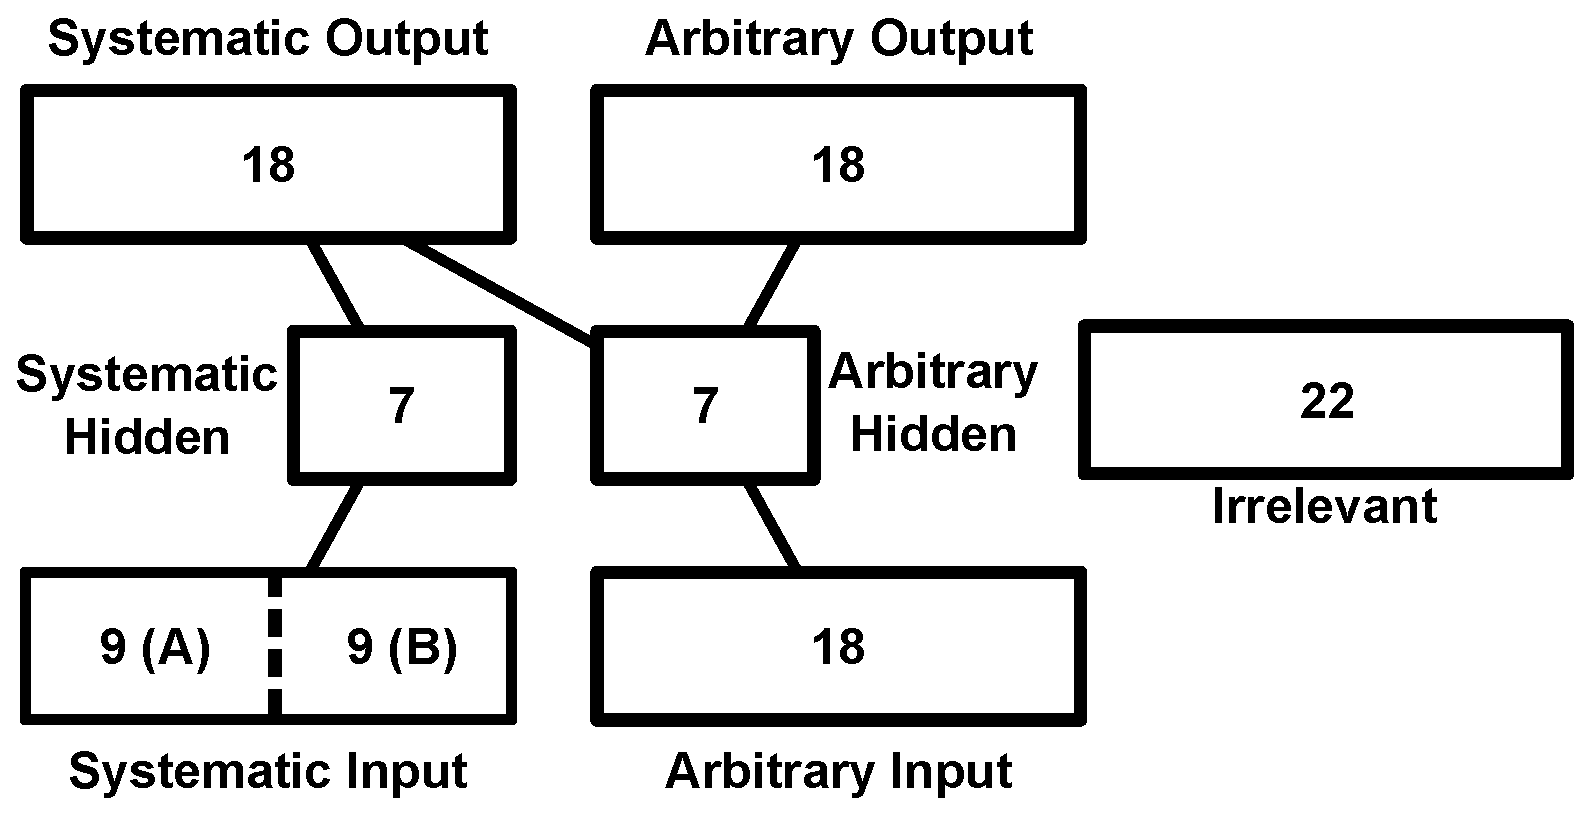
\includegraphics[width=0.75\textwidth]{figures/model_outline.eps}
\caption{\label{fig.sem_net} A schematic of the Rummelhart semantic network. Context sensitive and insensitive distributed representations of are learned for a set of examples. The structure of the distributed representations emerges because of coherent structure in how the model needs to respond to the various examples in each context. See \protect\cite{rogers_semantic_2004} for a full discussion of this model.}
\end{figure}


With this overview of how PDP models work, we are ready to consider the challenges that the PDP framework raises for the discovery of mental representations in functional brain imaging data. Many difficult issues arise, of course, in any effort to relate artificial neural networks to real neural networks. Because network models are functional abstractions of the neural processes they aim to uncover, they necessarily gloss the complexity, and many aspects of structure and behavior, known to be important in real nervous systems. Acknowledging the interest, import, and complexity of these issues, we here adopt a fairly simplified stance on the relationship between network models and the brain networks we seek to discover in imaging data. Specifically, we assume that the activation of a single unit in a network model is analogous to mean neural activity in a population of hundreds of neighboring neurons within a small volume of cortex as estimated at a single voxel from BOLD activity in fMRI. Thus we will treat the pattern of activation generated by a given stimulus over units in a model network as analogous to the set of beta coefficients estimated over voxels from the BOLD response evoked by a given stimulus in a sparse event-related design. 

Even with this relatively transparent view of the relation between model elements and measured physiological responses, PDP raises four difficult challenges for the discovery of representational structure in the brain.

\begin{APAenumerate}
\item The behavior of a given cortical subregion (i.e., voxel or voxel cluster) can vary substantially across individuals even if different individuals encode the same representational structure across the same general regions.

For any given network, there are typically many different weight configurations that can generate appropriate outputs given the various inputs. The particular configuration that a network discovers with learning can depend on many things, including the initial random weight configuration, the ordering and distribution of the learning experiences sampled from the environment, and the effects of noise in the unit activations and/or weight changes. Thus a particular hidden unit in a given model can, across different training runs in the exact same environment, exhibit quite different patterns of activation in response to a given input. Yet the internal representations learned by a network are not arbitrary; the learning models are of interest because they reliably extract important kinds of structure across the set of input and output patterns to which they are exposed. What varies is the particular way that individual units contribute to encoding the interesting structure across network runs.

It is worth noting that this consequence of distributed representations may pose greater problems for finding signal in some cortical regions than others. In peripheral regions (i.e., early sensory and motor cortices), it is clear that information is encoded in largely the same way, and with a largely similar neuroanatomical organization, across individuals. In association cortices, it may be that neural codes are more strongly shaped by learning and experience, so that the way information is organized across cortex is more highly variable. PDP models provide a rough analog to this state of affairs, insofar as input and output units for a given model are stipulated to represent information in the same way in every model training run---that is, in every model ``individual.'' The issues of variability in representation mainly apply to learned internal representations coded across hidden units.

\item Activation of individual units may not be interpretable independent of other units.

A corollary of the preceding points is that the behavior of a given cortical unit may not be interpretable, or may have quite different interpretations across individuals, when analyzed independently from other units. 
%A full consideration of the conjunctive qualities of distributed representations is beyond that scope of this article, but is explained well by \citeA{rogers_precis_2008}. Suffice it to say, that t
This property of distributed representation is important because it suggests that univariate approaches to data analysis--methods that assess the behavior of individual voxels or voxel clusters independently--can fail to uncover important components of neural representations. Wherever the interesting structure is embedded in activations across multiple cortical units, but is not reflected in individual units, such methods will yield null results.

\item The functional model architecture may not map transparently onto anatomical structure in the brain.

 A third issue concerns the relationship between the functional architecture of a computational model used to simulate performance on a task of interest and the actual anatomical structure of the corresponding neural network in the brain.  As noted earlier, units in PDP models are organized into layers, with units in a given layer receiving connections from and directing connections toward the same subsets of units elsewhere in a network. The layer is a useful construct for understanding how a network functions, insofar as the units within a layer, by virtue of having similar connectivity to the broader network, ``work together'' to represent and process the same information. Distributed internal representations in PDP networks are typically viewed, therefore, as being encoded across units within a particular layer.  

It may seem natural to view layers as model analogs of cortical regions, so that the gross architecture of a computational model maps transparently onto the anatomical structure of networks in the brain that carry out the modeled cognitive function. Though this analogy is reasonable, it is not the only possible way that the functional architecture of a computational model might relate to the neuroanatomical structure of a corresponding cortical network. In fact, the layers of a computational model do not, in principle, have any implications for how the corresponding cortical units might be anatomically situated in the brain. Units that function together as a ``layer'' could be situated in multiple different cortical regions, or widely dispersed anatomically, or interdigitated with other units subserving different functions. The defining property of layers in a computational model is their pattern of connectivity in the gross architecture, and the same network connectivity can exist among many different spatial arrangements of units [FIGURE?]. In other words, the relationship between the functional architecture of a computational model---the grouping of units into layers as typically depicted in model figures, for instance---may not transparently reflect the topological arrangement of the corresponding cortical units in the brain. 

This lack of transparency poses a problem for approaches to brain imaging that assume representations to be encoded over a volume of anatomically contiguous cortical units, including approaches that average signal over regions of interest, that spatially blur signal, or that restrict statistical analysis only to voxels within pre-specified areas. If cortical units that function together as a representational substrate do not happen to reside in a single contiguous cortical region, such methods may fail to discover important signal.

\item The network of interest in any given study co-exists in the brain with many other networks, all subserving other functions that may not be of interest.

Any given computational model is designed to aid understanding of a particular aspect of cognition, and typically includes only those elements that the theory stipulates to be important for the behavior of interest. Even if the model is a relatively faithful and accurate abstraction of a real cortical network in the brain, the physiological measurements generated by that network will, in any brain imaging study, be intermingled with measurements from a great many other cortical systems involved in other aspects of cognition unrelated to the task of interest. Since the tasks we study as cognitive neuroscientists tend to be comparatively simple, odds are that the great majority of measurements taken will reflect metabolic activity unrelated to the representational structure we are searching for. Thus the effort to find distributed representations in brain imaging data raises thoughts of needles and haystacks. If we cannot narrow the search by only considering contiguous volumes of units, or pre-selecting regions of interest, or reducing the complexity of the data by spatial smoothing, it is not clear how the needles are to be found.

\end{APAenumerate}

\subsection{Summary}
The representational assumptions of the PDP framework lead to the following somewhat bleak-seeming view. The behaviors of individual cortical units (read voxels) may not independently covary with or otherwise reflect the objects of representation we are interested in finding in a systematic way across individuals. Mental representations may instead inhere in the patterns of activation evoked across whole sets of units that together function as a representational ensemble by virtue of their connectivity within the overall cortical network (like the layers of a neural network model). This is the core sense in which representations are distributed in the PDP view. The way that a particular unit contributes to different representations can be highly variable across individuals, even if the ensemble encodes the same representational structure across individuals. This means that the search for voxels exhibiting similar responses in similar anatomical locations across people will fail to reveal important representational structure. Moreover, the units that operate together as a representational ensemble may not be anatomical neighbors, and are certain to be buried within the mountain of measurements provided by functional imaging technologies across the whole brain. These possibilities raise a daunting challenge: representational structure can only be discerned by considering the whole pattern of activation over a representational ensemble; yet the units within such an ensemble may be anatomically dispersed and intermingled with a vast amount of irrelevant information. One cannot understand the representation without knowing which units together constitute an ensemble, but how is one to find the ensemble in the first place?

In what follows, we assess how well different approaches to fMRI data analysis meet this challenge by applying them to the discovery of representational structure in data generated by a simple neural network model as it processes different input patterns. We will see that all methods bring with them important biases in the kinds of representational structure they are capable of detecting, and that some methods are better-suited to finding the distributed structure that the PDP framework assumes. We will also see that patterns of results across methods can provide important information about the nature of the representations encoded in different parts of a network.

\section{Model and Methods}

\textbf{---Figure 2 about here---}
\begin{figure}
\centering
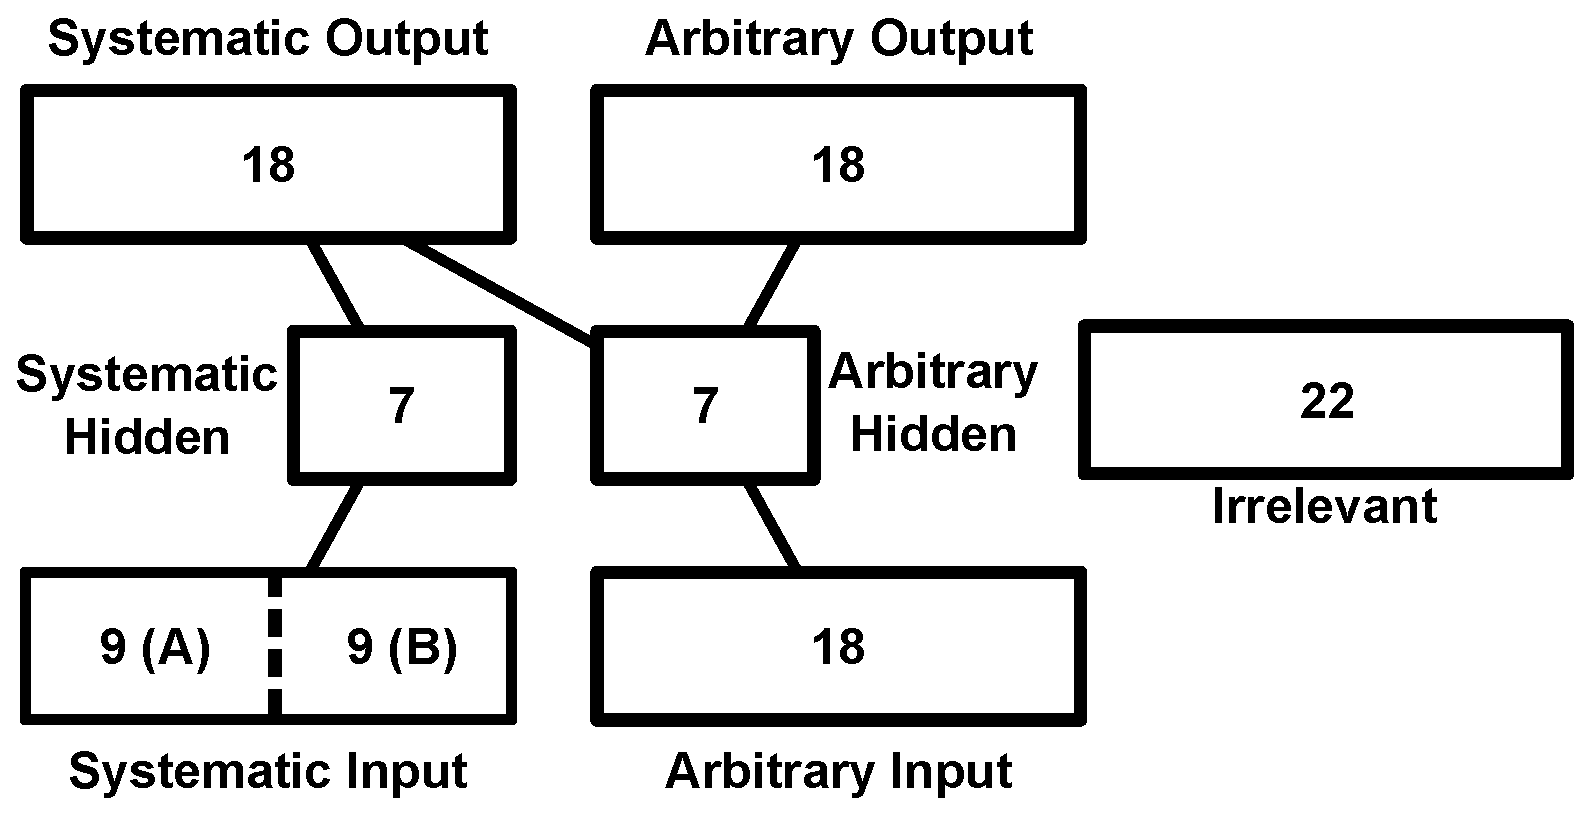
\includegraphics[width=0.75\textwidth]{figures/model_outline.eps}
\caption{\label{fig.model_outline} Schematic outline of the auto-encoder network used to generate the data for the 10 subjects used in subsequent simulations. The model has 36 input units (18 systematic), 14 hidden units (7 systematic), and 36 output units (18 systematic). The 22 irrelevant units are completely disconnected from the network, so receive no input, send no output, and thus learn no representations. They are intended to stand for units that participate in an unrelated network, which are nonetheless anatomically adjacent to our units of interest. See text for full description and motivation.}
\end{figure}


The model we will employ for this analysis is illustrated in Figure 2. It is an auto-encoder network: when presented with an experience in the form of a pattern of activity over its 36 input units, it learns to reproduce that same pattern over its 36 output units. Auto-encoder networks have been used as simple models of human memory, because once they have learned they are capable of both retrieving full information from a partial cue and of generalizing prior learning to new items. In this case, however, we do not intend the model to embody a specific hypothesis about a particular real-world cognitive function. Instead, the model is designed to make explicit the challenges noted in the introduction. 

To this end, the patterns that the model processes are viewed as coming from two different {\em domains}, A and B, corresponding to some cognitive distinction of theoretical import. For instance, A and B might correspond to nouns versus verbs, or animals versus manmade objects, or faces versus non-faces, or any other binary distinction thought to be of potential relevance to behavior.  Each individual item is represented with a unique pattern of activation over input units, and the network�s task is simply to generate the same pattern output units. In this sense, there is no explicit representation of the two classes A and B in the inputs, outputs, or network task. The two domains are assumed, however, to be distinguishable from the distribution of input/output properties they possess. Specifically, one subset of input/output properties is marginally more likely to be active for items from domain A, while another subset is marginally more likely to be active for items in domain B. We will refer to these subsets together as {\em systematic I/O} units, because they each weakly covary with the representational distinction of interest.  Each item also possesses many {\em arbitrary I/O} units that do not systematically differ between domains.

After the model has learned, it is possible to ``query'' it by presenting an input pattern and generating patterns of activation throughout the rest of the network. As noted earlier, we take the activation at each unit in response to an input as a model analog of the neural response to a stimulus estimated from the BOLD signal at a single voxel in a single individual. Across different training runs, the model will always exhibit the same overt behavior (generating the correct pattern over output units), but arising from different configurations of weights, and hence from different internal representations. Variability in weight configurations and internal representations acquired across different training runs thus provides a model analog of individual variability in the neural representations acquired across the population. To simulate data generated by a functional brain imaging study with, say, 10 participants, we train the model 10 times, and for each trained model, record the pattern of activation generated over all model units by each input pattern (i.e., stimulus).  The question we then wish to ask, by applying different statistical methods to the analysis of this synthetic imaging data from a sample of trained models, is the following: where are representations of the domains A and B encoded in the network?

The network architecture is designed so that there are two possible answers to this question. The first answer is that representations of A and B are directly encoded in the activations of systematic I/O units. For all input and output units, the response of a given unit to a particular item is directly specified by the environment, so that these units will always respond to a given stimulus in the same way across training runs. Each systematic I/O unit has a marginally different probability of being active depending upon the domain; in this sense the A units each independently encode a representation of the A domain and the B units encode a representation of the B domain. The relationship between domain and activation is, however, stipulated to be quite loose: for any A item, many A units will be inactive (and vice versa), and so each unit participates in few patterns. Thus different items in the A domain have quite different representations over A units, and the correlation between activation and domain is weak for any individual unit. Nevertheless, each input and output units responds to stimuli in exactly the same way across model individuals (subject to noise in measurement as explained below). We further stipulate that the A input and output units are anatomical neighbors, as are the B input and output units, and that this anatomical arrangement is exactly the same across individuals. Thus the systematic I/O units individually encode a {\em weak} distinction between A and B that is {\em consistent} across model individuals and is {\em anatomically localized} within input and output layers. 

The second answer is that the representations of A and B domains are encoded in a distributed fashion over a subset of model hidden units. As shown in the Figure, the input units project to the output units by way of two separate hidden layers. The {\em systematic hidden layer} (SH) contains 7 hidden units that receive connections from the systematic input units and send connections to the systematic output units. The {\em arbitrary hidden layer} (AH) also contains 7 units that receive connections from the arbitrary inputs, and send connections to {\em both} the systematic and arbitrary outputs.  The weights are shaped by learning, so each input generates a pattern of activation over both the SH and AH layers, each corresponding to a learned internal representation of the stimulus. The particular way that layers are connected, however, ensures that these internal representations will have specific representational properties. Because SH layer only passes activation from systematic input to systematic output units, it uses it's limited representational capacity to capture the A/B distinction as best it can---items within a domain are represented by quite similar patterns relative items between domains. In contrast, the AH layer receives inputs only from the arbitrary input units and thus uses it's own limited representational capacity to differentiate between each of the items. Consequently, the AH layer acquires distributed internal representations that have very little structure; and the weights in the arbitrary pathways serve to ``memorize'' both the arbitrary features and the idiosyncratic ways that each item differs from its neighbors in systematic properties. In other words, the architecture produces a division of labor in which the SH learns distributed representations that emphasize the A/B distinction, and the AH does not. A good method, then, should identify SH units as important for representing the domains.

In addition, there are 22 completely irrelevant units. These units are positioned anatomically adjacent to the SH and AH units but are completely unrelated to the behavior of the network. Because they receive no input, they never activate. They are nevertheless important to the simulations that follow: they stand for units that participate in some other network altogether, yet are anatomic neighbors to the SH and AH units. Acknowledging challenges 3 and 4, these units are also measured, and might even be interspersed with the representations we care to discover.

\textbf{---Figure 3 about here---}
\begin{figure}
\centering
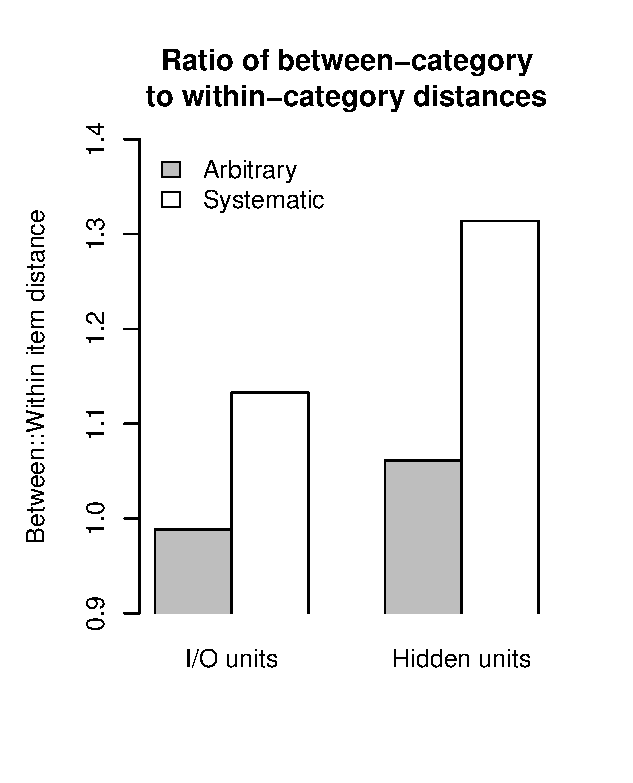
\includegraphics[width=0.5\textwidth]{figures/between_within_dist.eps}
\caption{\label{fig.between_within_dist} The dissimilarity of two distributed representations can be quantified as a distance. Distributed representations that have large distances between items from domains A and B in our model, relative to the distances between items of the same domain, will contain information relevant to training a classifier to determine which domain an example belongs to. Here, we plotted the ratio of between::within group distances for the representations over different sets of units in our network, averaged over the 10 subjects used in subsequent analyses. }
\end{figure}

With this general understanding of the model behavior, let's consider how it makes explicit the four challenges for brain imaging noted earlier. First, although the same representational structure is observed across all network runs, the particular way it is expressed across individual units is essentially arbitrary for the reasons noted in the introduction (challenge 1). Second, the mean activations of SH units taken independently do not systematically differ for items in the A and B domains: to find the important structure, one must consider the pattern evoked over multiple units (challenge 2). Third, the functional architecture of the model shown in Figure 2 can be anatomically arranged in many different ways (challenge 3). To make this issue explicit, we consider two different topographic arrangements of the functional model. In the first, units within the same layer are always situated as anatomical neighbors, so that the representations encoded by the SH and the AH layers are {\em anatomically localized}. In the second arrangement, we assume that the SH units are {\em spatially intermingled} with the AH units, in a different way across model individuals, so that the representations they encode are {\em anatomically dispersed}. In the results we will consider how well each method identifies the SH units as a function of whether they are localized or dispersed. Finally, the model captures the idea that the units of interest constitute only a small proportion of all the units measured (challenge 4). In the model itself, most of the units are dedicated to processing arbitrary patterns (18 arbitrary I/O units and 7 arbitrary hidden units). The next largest set of units that participate in the network are the systematic I/O units that weakly but consistently encode the category structure. The units of greatest interest, the SH units, constitute just 6\% of all the units in the data. 

\subsection{Summary} 

Though very simple, this auto-encoder network captures each of the challenges noted in the introduction: it acquires distributed internal representations that express representational structure of interest; the way the structure is coded across units varies in different individual models; the structure cannot be discerned from the activations of single units but arises in patterns over multiple units; the relationship between the functional architecture and the underlying model topography can be opaque; and the units that encode the structure we wish to discover are buried in a large number of other measurements. The question we now address is how well different analysis methods fare at discovering representational structure across both systematic I/O units and the SH units, when they are applied to data generated from a sample of model training runs.

\section{Simulation details}
The model outlined above has 36 input units (18 systematic), 14 hidden units (7 systematic), 36 output units (18 systematic), and 22 irrelevant units that do not receive any inputs or outputs. The model's environment consists of 72 input patterns, which are sampled from two domains, distinguishable based on their systematic input. Half of the input patterns activate units from the first 9 systematic input units (domain A items) and the other half activate units from the second 9 systematic input units (domain B items). The construction of these input patterns was carefully balanced, so that every pattern consisted of exactly 2 systematic and 2 arbitrary input units, that every unit was active in exactly 8 input patterns. Arbitrary units were balanced as closely as possible with respect to category. This all ensures that systematic input units are equally weakly informative about what category a thing belongs to, and that arbitrary units are devoid of category information.  

The model was fit in LENS \cite{rohde_lens:_1999} using back-propogation to minimize cross-entropy. The weights were adjusted with momentum and subject to weight decay which decreased the size of all weights by 0.1\% after every epoch. The model was trained 10 times to asymptotic performance with very low error over 1000 epochs. These 10 models were used to generate data for 10 ``subjects'', based on the patterns of activity over the whole network in the presence of each item. Despite being trained on exactly the same 72 items and obtaining the same level of performance, each model learned different internal representations over their hidden units. Each subject's data set is a 1-dimensional vector of values, arranged from the first input unit to the last output unit. Prior to any reordering, the data for each subject contains well localized signal that is consistently located across subjects.

These 10 datasets contain the ``true'' response pattern for each subject to each item. In any real application, true signal is buried in noise. Of course, the properties of this noise and the signal to noise ratio are important considerations in reality; they will be handled very simply in these simulations. All true activation ranges from 0 to 1, and we added a i.i.d Gaussian random value to each unit, N(0,1). 

\section{Results}

With this understanding of the model, we are now ready to consider how different statistical methods for fMRI fare at discovering the model units that encode representations of the two domains, both in the case where the hidden units are anatomically localized and when they are anatomically dispersed. The methods we consider include the standard univariate contrast method and four forms of multivariate pattern classification (MVPC). Each method faces the challenges inherent in fMRI analysis--that of finding meaningful signal within a vast amount of quite noisy data. To address the challenge, each method adopts a different set of assumptions about the nature of the underlying signal, and so brings with it biases in the kinds of results it yields. For each method, we will begin with a brief exposition of the basic logic and essential concepts and will explicitly note the underlying representational assumptions. We then report the implementational details and results of the analysis, with the aim of answering four questions:

\begin{enumerate}
\item Does the method identify the systematic I/O units, but not arbitrary units, as important for domain representation?
\item Does the method identify the systematic hidden units, but not arbitrary units, as important for the domain representation?
\item Do the results differ when hidden units are anatomically localized versus dispersed?
\item Does the method indicate differences in how the information of interest is coded across unit sets? Specifically, does it indicate that some units respond more to A items than to B items, others show the reverse pattern, and still others express the A/B distinction with a distributed code? 
\end{enumerate}

\subsection{Univariate contrast analysis}
\subsubsection{Concept and assumptions} The univariate contrast analysis is the standard method for interrogating fMRI data. The goal of the method is to identify regions of cortex that, across subjects, exhibit systematically different mean BOLD responses to two (or more) different kinds of cognitive events. Typically the BOLD signal is spatially smoothed, so that the raw response at each voxel is replaced with a weighted average of the responses from anatomically neighboring voxels. The smoothed time-series is then modeled independently at each voxel for each subject using a deconvolution procedure. This yields a beta coefficient for each experiment condition at each voxel indicating how well the measured BOLD signal matches the response expected if the activation of neurons within the voxel varies systematically with the experiment condition. The beta coefficients for each subject are projected into a common anatomical reference space, and univariate statistical tests are computed at each voxel independently to assess whether the coefficients differ reliably in the two experimental conditions across subjects. Voxels that show significantly different responses across subjects are viewed as important for coding the representation of interest. 

A major challenge for the approach lies in establishing a meaningful criterion of significance in the context of tens or even hundreds of thousands of individual statistical tests. To avoid both false-positives and punishing corrections for multiple comparisons, it is common to seek ways of reducing the number of tests performed. Several different methods have been employed, but all rely on the idea that the representations of interest can be localized to particular cortical regions, and that the responses of voxels within a functional region will be largely similar. With these assumptions, the number of tests can be reduced by 
\begin{seriate}
  \item conducting regions-of-interest analyses, where the responses of voxels within a ROI are averaged and the test is performed on the result mean response,
  \item applying cluster-thresholding, where tests are only performed on clusters of {\em n} anatomically contiguous voxels all showing a similar response across subjects, or
  \item applying a topographic control of the false-discovery rate. 
\end{seriate} 
The univariate contrast method thus favors the discovery of clusters of anatomically neighboring voxels located in similar regions across individuals and showing similar response profiles across experimental conditions. 

From this brief description we can see that the method relies on five assumptions about the nature of the neuro-cognitive representations:

\begin{enumerate}
\item Localization within individuals: Representations are anatomically localized within individuals, so that neighboring voxels all contribute to the same representation.

\item Consistency of coding within individual representations: Within individuals, voxels contributing to a given representation encode the same information in the same way---for instance, always showing greater activation for one condition relative to another.

\item Localization across individuals: A given representation is encoded in anatomically similar regions across individuals.

\item Consistency of coding across individuals: A voxel at a given anatomical location will code the same information in the same way across individuals.

\item Independence of representational units: The interpretation of a voxel's activation does not depend on the states of other voxels.
\end{enumerate}


Assumptions 1 and 2 license spatial smoothing of the raw BOLD signal, a data processing step that will only improve signal if these are both valid. Assumptions 3--5 license the logic of the general approach--that of seeking single voxels in similar anatomical locations across individuals that exhibit a similar pattern of contrasts across experimental conditions. The five assumptions together license the common methods for dealing with the vast amount of data by reducing the number of statistical tests performed. 

With these assumptions, what does the univariate contrast approach discover in the model?

\subsubsection{Implementation}
The activity at each unit was modeled simultaneously for all subjects in a mixed effects model that treated subject as a random factor \cite{chen_linear_2013, friston_mixed-effects_2005} using the lme4 package in R \cite{bates_linear_2013}. Each model contains a single regressor, coding whether each item is an example of category A or B. The coefficients obtained from the mixed effects model were tested for significance using the Kenward-Roger approximation for the degrees of freedom \cite{kenward_small_1997} and a standard F-test, numerator degrees of freedom = 1, denominator degrees of freedom = 9. The results are directly analogous to a repeated-measures ANOVA. The criterion for significance, alpha, is corrected to control the false discovery rate at q<0.05. 

For this and all other methods, the analysis was conducted twice. The first time, the data were assumed to be generated by a network with the same topographic structure shown in Figure \ref{fig.model_outline}. That is, the systematic hidden units were anatomical neighbors, as were the arbitrary hidden units. The second time, the data were assumed to be generated from a network in which the anatomical location of the hidden units was permuted so that the systematic hidden units were randomly interspersed among the arbitrary hidden units and 22 irrelevant units. In both cases, the data were smoothed, taking a weighted average over a three unit window, where the center unit was weighted about twice as much as the two flanking units.

\subsubsection{Results} 
\textbf{---Figure 4 about here---}
\begin{figure}
\centering
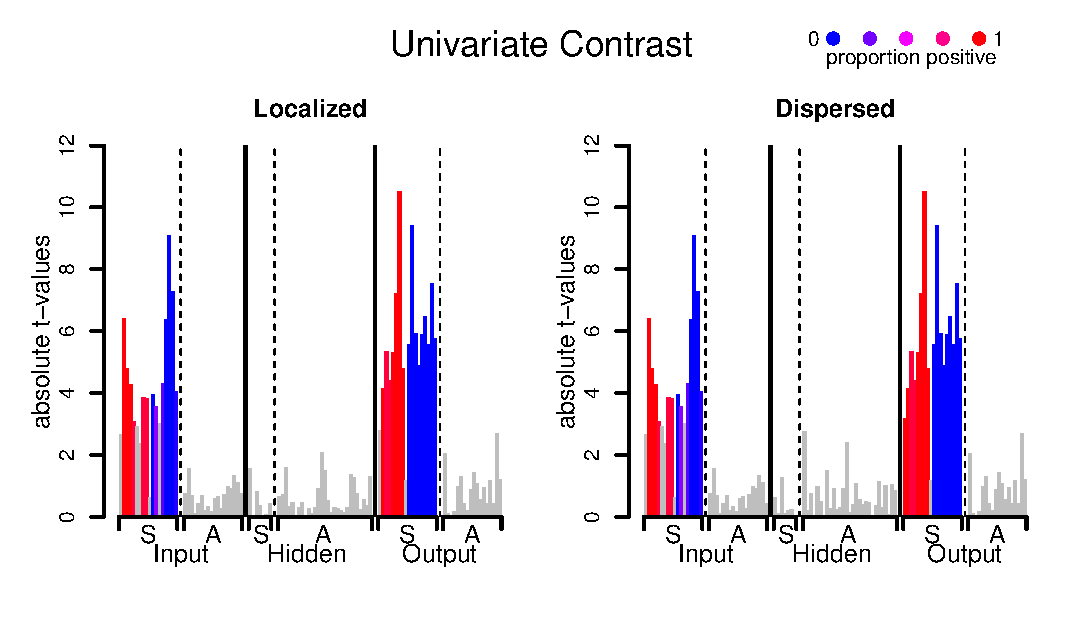
\includegraphics[width=0.75\textwidth]{figures/univariate.eps}
\caption{\label{fig.univariate} Results from the univariate analysis of simulated data. Bar height indicates the t-value of the voxel-wise contrast between conditions at the group level. Bars in red are significant, p-values corrected to control the false discovery rate at $q<0.05$. In all plots, the distributed condition is created by permuting the units within the hidden layer. For plotting, results are un-permuted back to their original order.}
\end{figure}

Figure \ref{fig.univariate} shows the results of applying the univariate method to the localized (left) and dispersed (right) models. In these plots, each bar corresponds to a single unit in the model (analogous to a single voxel). The bars are ordered according to their functional role in the network, as indicated by the X-axis labels. Colored bars indicate units showing statistically significant differences in mean activation across model individuals, while grey bars indicate units that did not show significant differences. Among the colored bars, red indicates units where activation was reliably higher for domain A, and B indicates units where activation was reliably higher for domain B. Note that, in the ``dispersed'' plot (right), the units are shown in their standard functional location for ease of interpretation.

In both localized and dispersed cases, the univariate contrast method identifies systematic I/O units as important for representing the A/B distinction, and correctly indicates that different subsets of input units code this information differently (some responding more to A than B and others showing the opposite pattern). Note that these are the units for which the five univariate assumptions about representation are all valid. In both localized and dispersed cases, however, the analysis completely misses the systematic hidden units, even though these jointly encode a cleaner representation of the A/B domain structure. The failure arises because, in both cases, the univariate assumptions are invalid. When hidden units are localized, assumptions 2 and 4 are violated: the way individual units encode information can vary across SH units in the same model individual, and across individuals at the same anatomical location. When the units are anatomically dispersed, assumption 3 is also invalid: the representation is coded in different anatomical locations across individuals. Because of these departures from the statistical assumptions, the mean activation of a unit at a given anatomical location across individuals does not differ reliably for SH units, even though these do reliably encode the domain distinction in each individual.

In summary, we get the following answers to the core questions:

\begin{enumerate}
\item \bf{Does the method reliably identify the systematic I/O units?} Yes.
\item {\bf Does the method reliably identify the systematic hidden units?} No.
\item {\bf Does the method indicate how the information of interest is coded across identified units?} Yes.
\item {\bf Do method results depend on anatomical localization of signal-carrying units?} No---hidden units are not discovered regardless of anatomical layout.
\end{enumerate}

\subsection{Multivariate pattern classification}

The remaining methods we consider are all multi-voxel pattern analyses (MVPAs). As a class of methods, MVPAs reverse the objective relative to univariate analyses. Rather than using knowledge of the experimental design to explain variance in neural activity at individual voxels, MVPAs use the variance of neural activity in many voxels to 
make predictions about which experimental condition each trial/stimulus/time point (henceforth, ``example'') belongs to \cite{mitchell_learning_2004, pereira_machine_2009}. To accomplish this, three things are necessary: 
\begin{seriate}
  \item a set of {\em training data} to be trained on, arranged in a matrix with one column per voxel and one row per example,
  \item a list of {\em labels} that identifies each example with a condition or other meaningful division within the data, and
  \item a classification algorithm, of which there are many to choose from.
\end{seriate}
The training data will be a subset of the full dataset, intentionally excluding some examples so they can be used to evaluate how well the trained classifier generalizes. The set of examples withheld for this purpose is called a {\em hold-out set}. This procedure of training on one part of the data and testing on another is called {\em cross-validation}. Cross-validation can be done several times, each time with a different hold-out set---this is done to ensure that results do not depend upon a particular configuration of training and hold-out sets, and is called {\em n-fold cross-validation}. Each hold-out set provides a measure of classification accuracy, which can be averaged together to obtain the {\em mean cross-validation accuracy} for classifiers trained on a certain set of voxels.  

Cross-validation is important because training data can be well modeled even in cases where no true relationship exists between the training data and the labels. In such a case, which is more likely to occur as the number of voxels in the training set increases, classifier performance {\em on the training set} will be good, but it will fail to generalize.  When cross-validation accuracy is better than chance, it indicates that the classifier is exploiting real relationships between neural activity and the conditions rather than just fitting noise in the training set.
 
However, in any fMRI study (as in our model) there will be more predictors (voxels) than things predicted (examples). In such cases, no unique solution exists; closed-form analyses are undefined, and other model-estimation procedures will produce a classifier that perfectly fits the training data without any guarantee of finding real signal.  This problem is called ``over-fitting'', and it can be addressed only by constraining the analysis based on an underlying hypothesis about how signal is truly encoded in the data. As was the case with the univariate method, these constraints systematically affect the results. Each of the remaining methods adopt different constraints to solve the over-fitting problem.

\subsubsection{Searchlight concepts and assumptions}
We begin with the well-known ``searchlight'' approach \cite{kriegeskorte_information-based_2006}, which was formulated specifically to address the challenge of finding distributed representations in brain imaging data. The method works as follows. Instead of training a classifier using all predictors at once, a separate classifier is trained for every individual voxel location in every individual subject. For each location, all voxels within a radius $r$ of the center voxel are included as predictors in the classifier. This avoids the over-fitting problem by restricting the number of predictors included in any given classifier.  The mean cross-validation accuracy for each classifier is stored in the searchlight center voxel, providing an ``information map'' for each subject. After deriving information maps, a univariate group-level analysis can be conducted on these maps, similar in all respects to the analysis described in the previous section. In sum, the method will flag as ``significant'' clusters of voxels that reside in similar locations across individuals and that, together with their anatomical surround, yield above-chance classifiers.  

With this brief overview of the approach, it is useful to consider how the searchlight assumptions about representation compare to those of the univariate method:
  
\begin{enumerate}
\item Localization within individuals: For a classifier to show above-chance cross-validation accuracy, there must be sufficient information contained within its searchlight. If the representation is anatomically distributed such that no searchlight contains sufficient information, the method will not discover the representation. In this sense, the method assumes localization of the representation within individuals, similar to the univariate case.

\item Consistency of coding within individual representations: In contrast to the univariate approach, the method does {\em not} assume any consistency in how information is encoded across voxels within a representation for a given individual. Different voxels contributing to the same representation can respond to various stimuli in quite different ways. So long as the information is present within the searchlight, the classifier can exploit it.

\item Localization across individuals: Like the univariate method, the searchlight approach assumes that the representation will be localized in similar ways across individuals. This assumption licenses the cross-subject test of classifier accuracy at each voxel. If representations are localized differently across individuals, the searchlights that yield above-chance classifications will reside in different anatomical locations in different subjects, so the statistical tests across individuals at common locations will yield null results.

\item Consistency of coding across individuals: In contrast to the univariate case, the approach makes no assumptions about the nature of the code at a given location across individuals. So long as a given location contains information relevant to the classification, the method will detect it, regardless of how the information is coded.

\item Independence of representational units: Unlike the univariate case, the approach does not assume that voxel activations can be interpreted independently. Searchlight classifiers operate on patterns of activation across units in the searchlight, so the effect of a given unit on the classification can differ depending upon the activations of other units in the searchlight. The method does assume, however, that each searchlight can be interpreted independently of every other searchlight. If the information coded in one searchlight varies depending upon the states of units in other searchlights, the method will not discover this.
\end{enumerate}

Thus the searchlight method relaxes assumptions about the consistency of the neural code within and across individuals, and about the independence of representational units, but retains assumptions about localization of information within and across individuals. What results are observed in the model with these differing representational assumptions?

\subsubsection{Implementation}
The searchlight analysis was conducted using the SearchMight toolbox \cite{pereira_information_2011} for Matlab\textregistered (Mathworks, 2013a). To ease interpretation, each layer was treated as a separate anatomic region. This was accomplished by inserting empty units between the layers, and providing a mask to SearchMight to omit those units during analysis while ensuring that no searchlight spans multiple regions. Within each searchlight, a Gaussian Naive Bayes (GNB) classifier was fit to distinguish between category A and B items. Although GNB classifiers are limited in some ways \cite{pereira_information_2011}, the concerns do not apply to this simple and idealized case where noise is truly i.i.d. with uniform variance. The amount of category information in each searchlight was estimated through 6-fold cross validation; the mean cross-validation accuracy was stored at each searchlight center; and the mean accuracy over model subjects was then computed for each unit and tested to see if it differed significantly from chance. The resulting map of p-values is FDR corrected, q<0.05.

As previously, the analysis was performed on both the anatomically localized and the anatomically dispersed arrangements of units. Because the searchlight method effectively ``smooths'' the data by looking for information over multiple neighboring units, the data were not smoothed prior to the searchlight analysis. The analysis was performed with various searchlight sizes, ranging from 3 to 28. A searchlight size of 7 or 9 should be roughly ``optimal'' given the size of the clusters of informative units in the localized data.

\subsubsection{Results} 
\textbf{---Figure 5 about here---}
\begin{figure}
\centering
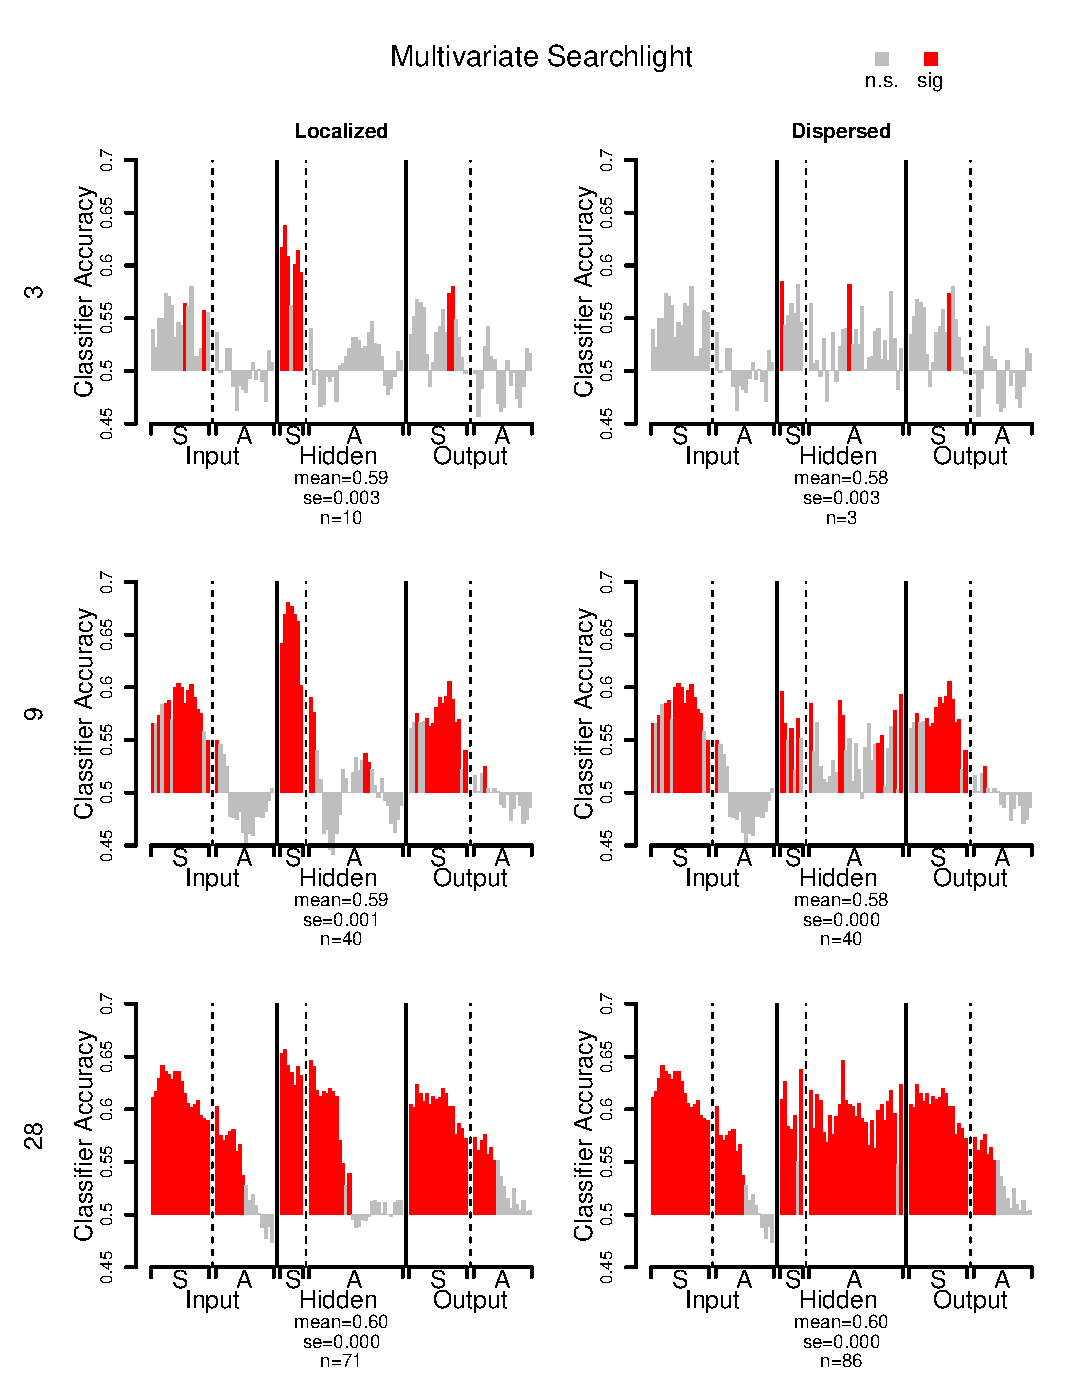
\includegraphics[width=0.75\textwidth]{figures/searchlight.eps}
\caption{\label{fig.searchlight} Result of the multivariate searchlight analysis of simulated data. Bar height indicates the mean classifier accuracy over subjects. Bars in red indicate searchlights where classification accuracy differed from chance over subjects, p-values corrected to control the false discovery rate at $q<0.05$. Results are presented for the searchlight sizes, indicated at the far left of each row.}
\end{figure}

Figure \ref{fig.searchlight} shows the results of the searchlight analyses, for localized and dispersed model architectures, and for different searchlight sizes. The format is the same as in the preceding analysis, except the y-axis now indicates the mean classification accuracy for spotlights centered on each unit, rather than a t-value at each unit. As before, colored bars indicate units that the method identifies as statistically significant---that is, units whose surrounding searchlights show classification accuracy reliably above chance across model individuals.

There are several points to note in these plots. First, when the hidden representations are anatomically localized, the method can do a quite good job of identifying both the systematic I/O and the systematic hidden units as important for the domain representations, though for both unit types the results vary substantially with the spotlight size. When the spotlight is small, the method reliably finds the SH units but misses most of the systematic I/O units. This happens because, as noted earlier, the SH units encode a clearer differentiation between domains, so that even if the spotlight does not encompass all 7 units there is sufficient information within it to classify stimuli above chance. The domain distinction is weaker in the systematic-I/O units, so when only a small number of such units fall within the spotlight, there is insufficient information to classify correctly. With a larger searchlight (9 units), the method does very well at finding all relevant units.  When it grows too large, however, it begins to incorrectly flag irrelevant units as being important for the representation (28 units). A very large spotlight, even when centered on an uninformative (arbitrary) unit, can have a broad enough span that it encompasses other informative units. In this case the classifier will perform well by virtue of the informative units appearing in the edge of the spotlight, but the above chance result will be ``stored'' in the spotlight center, making it appear as though there is useful information present at that location. Thus when the signal is anatomically localized, there is a tradeoff between spotlight size and discovery of representational structure, with spotlights that are too small missing weaker signal and those that are too large incorrectly flagging arbitrary signal.

In the model case, where we know {\it a priori} which are the signal-bearing units, it is easy to discern the optimal searchlight size, but it is less clear how this would be determined from real brain imaging data. One might initially expect the optimal searchlight to be identifiable from the accuracy of the resulting classifiers, but Figure \ref{fig.searchlight} suggests that this is not the case: the very large searchlight, which flags many irrelevant units, shows almost as good classifier performance as the optimal size at the SH units and better performance at the systematic I/O units. If we did not already know which units were important for representation in the model, it would be difficult to know which searchlight size to choose, and hence which results to believe.

The second thing to note is that the searchlight analysis does a much poorer job overall of identifying the SH units when these are anatomically dispersed (right panels of Figure \ref{fig.searchlight}). The poor performance arises because the precise anatomical location of the signal-carrying units is assumed to vary across individuals in this case. Within any individual model, a searchlight that includes a few of the informative units will show above-chance performance in classification, but the searchlight centers will differ across model individuals, especially when the searchlights are small. Thus the cross-subject statistical test at each location will yield a null result, leading to poor signal discovery. Larger searchlights will be more likely to contain the signal-carrying units, but also lead to poorer localization of the signal as already noted. 

In sum, the method deals with the over-fitting problem by only including a small number of contiguous voxels in each classifier---an approach which assumes that useful representational structure can be localized within the searchlight radius, in the same locations across subjects. When these assumptions are met, the approach does a good job of discovering representational structure, even if the representational code (i.e., the way that individual units respond to particular stimuli) is highly variable within and across individuals. The limitations noted above arise when the assumptions are violated---when representational structure is anatomically distributed across multiple spotlights (as when spotlights are too small in the localized case), or in different ways across individuals (as in the dispersed model). Moreover, whether the assumptions are met depends, not only upon the anatomical distribution of the signal, but also upon the searchlight size, and it is not clear how the latter can be optimized for real brain imaging data.  

Finally, it is worth noting that, in contrast to the univariate method, the searchlight approach does not provide information about how the contrast of interest in encoded in unit activations. Each searchlight returns a single number indicating how well its surround differentiates items from the two classes, but it does not indicate how the distinction is encoded in unit activations. Thus there is no way for the method to show, for instance, that there are some units systematically more active for A items than B items, others showing the reverse pattern, and still others that express the A/B distinction in a distributed code (the SH units).

Returning to the central questions, we get the following answers:

\begin{enumerate}
\item {\bf Does the method reliably identify the systematic I/O units?} Yes, though results vary substantially with searchlight size.
\item {\bf Does the method reliably identify the systematic hidden units?} Yes, when they are anatomically localized and when the searchlight is not too large.
\item {\bf Does the method indicate how the information of interest is coded across identified units?} No.
\item {\bf Do method results depend on anatomical localization of signal-carrying units?} Yes: performance declines substantially when signal-carrying units are anatomically dispersed.
\end{enumerate}

\subsection{Regularized logistic regression for whole-brain pattern classification}
\subsubsection{Concepts}
The limitations of the searchlight method arise from the relationship between a searchlight's field of view and the anatomical distribution of the underlying signal. A small searchlight provides better localization but is more likely to exclude signal-carrying units; a large searchlight is more likely to include the signal-carrying units but provides less information about where the signal really is. An alternative approach that avoids this tradeoff is to train a pattern classifier on the whole dataset simultaneously, as if we were using one giant searchlight, and to use the resulting statistical model (the set of weights learned by the classifier) to understand how each unit contributes to the overall solution. For instance, units with weights of zero contribute nothing to the classifier ``decision'' and so are identified as unimportant for the contrast of interest. Moreover the sign of the weight might indicate how units activations are to be interpreted. In a binary contrast of conditions A and B, where A events are labeled with 1 and B events are labeled with 0, then positive weights on a unit suggest that higher unit activation provides evidence for condition A while negative weights suggest that higher activation provides evidence for condition B. Thus the classifier cross-validation accuracy indicates whether the classifier has discovered true signal, and the weights indicate how the underlying signal can be interpreted, all without making any assumptions about the anatomical relationships among the signal carrying voxels.

Logistic regression provides one form of classifier that is a natural candidate for this sort of analysis. Standard logistic regression can be viewed as an optimization that seeks a set of coefficients (predictor weights) minimizing, across all items in the training data, the discrepancy between the model output and item labels. Let the item labels be represented by $y\in{\left\{0,1\right\}}$.  This discrepancy can be quantified by the logistic loss function:

{\em  formula here?}
\begin{align}
f(z) = \frac{e^z}{1+e^{z}}
\label{eq.logisticloss}
\end{align}

Where $z = \beta_0 + \beta_1X_{i 1} + \beta_2X_{i 2} + \dots +  \beta_1X_{i n} + e_{i}$, and $f(z)$ can be interpreted as the probability that $y=1$ given the pattern of activity for the $i^{th}$ item. 

As noted previously, the problem is that there are infinite possible solutions to the minimization when there are more predictors than items. One needs a way of deciding which among these is most likely to uncover the real signal. {\em Regularized} regression provides one way of doing this. Such approaches seek to jointly minimize the logistic loss (i.e., error in prediction) plus an additional cost, itself a function of the coefficients:

{\em  equation?}
\begin{align}
\hat \mathbf{w} = argmin{w} \left( \sum^n_i{\left(y-f(z)\right)^2 \right) + \lambda h(x)
\end{align} 

The additional penalty or {\em regularizer} essentially "prioritizes" some model solutions over others, and in this way embodies a hypothesis about the nature of the "true" underlying signal. The constant $\lambda$ is a free parameter that controls the degree to which the two terms (prediction error versus minimization of the regularizer) should be weighted in the joint optimization.

We here consider two varieties of regularized logistic regression recently employed in the fMRI literature \cite{XX}: L1-regularized regression or LASSO, and L2-regularized or {\em ridge regression}. Though superficially similar, the two methods embody different implicit assumptions about the nature of the underlying signal and so yield quite different results. In LASSO, the regularizer is the L1-norm of the coefficients, that is, the sum of their absolute values:

{\em  equation here}

For ridge regression, the penalty is the L2-norm of the coefficients, that is, the sum of their squared values:

{\em  equation here}

In both cases, any predictor that carries no information at all about the category label should receive a zero weight, since this minimizes the predictor's contribution to the regularization penalty and without affecting the prediction error. In this sense, both methods can be viewed as "weeding out" irrelevant predictors. Apart from this similarity, however, the penalties behave very differently. To understand why, it is useful to consider how they treat sets of predictors that covary together with one another. Imagine 4 voxels whose responses across items are perfectly correlated, and suppose their activations are useful in predicting the condition label. In this scenario, there are many different ways of placing weights over the 4 voxels that will all have the same effect on the classifier output. For instance, placing a weight of 1 on each voxel will have exactly the same effect as placing a weight of 4 on one voxel and a weight of 0 on the other three. Because the voxel activations are perfectly correlated, and the classifier operates on a weighted sum over voxel activations, these different weight configurations have the same effect on the model output and hence on the prediction error. The regularization penalty, however, should prefer some weight configurations over others.

If the data really are perfectly correlated, the LASSO penalty won't be any help: the sum of the absolute value of the coefficients is the same for models that place a 1 on each unit versus models that put a 4 on one unit and zeroes on the rest. If we imagine, however, that all measurements are subject to some independent noise, the scenario is a bit different. In this case, one of the 4 units will, just by chance, covary slightly better with the category labels. In this case, the classifier can do a slightly better job of minimizing the error term by loading up all of the weight on this single voxel. Thus the joint optimization will lead to a solution where just one (or perhaps a few) of the redundant voxels are selected. Ridge regression behaves very differently. Here the penalty scales exponentially as weights increase on a single voxel, but only linearly as weights are added across voxels. Thus the penalty is minimized by placing small weights on many voxels. In the preceding example, placing a weight of 4 on one unit and 0 on the remaining 3 leads to a total penalty of 16 over the 4 units. Placing a weight of 1 on each unit, in contrast, leads to a penalty of 4. Ridge regression thus prefers solutions where small weights are "spread out" over redundant predictors. In fact, as the weight approaches zero, the ridge penalty becomes vanishingly small, so ridge regression will always place a tiny weight on any predictor that carries even very weak information about the label. In real data, of course, voxel states are never perfectly correlated nor perfectly informative about the condition label, so the behaviors of the two approaches are less easy to intuit. In general, however, it is useful to think of LASSO as minimizing prediction error with the {\em fewest} possible predictors (ie, as many zero coefficients as possible), while ridge regression can be viewed as "spreading" small weights over all predictors exhibiting any systematic relationship with the category labels, without care for the number of predictors. 

What assumptions do these approaches then bring about the nature of the underlying representation? Let's first consider the univariate assumptions: 

\begin{enumerate}
\item Localization within individuals: Both methods operate on all voxels at once and are blind to anatomical relations among voxels, so no localization is assumed.

\item Consistency of coding within individual representations: Both methods allow for the placement of any weight on any voxel so there is no assumption that information is encoded in the same way across representational elements.

\item Localization across individuals: These analyses are intrinsically single-subject analyses: each classifier is trained and test on each participant individually, and each participant yields a unique solution. Thus no localization across individuals is assumed

\item Consistency of coding across individuals: Because the analyses are applied separately to individual subjects, no consistency of coding across individuals is assumed.

\item Independence of representational units: Classifier outputs operate on patterns of activation elicited over the whole brain, so the approach does not assume that activations of individual voxels, or even sets of voxels within particular cortical regions, can be interpreted independently.
\end{enumerate}

These approaches thus relax {\em all} of the univariate assumptions (and likewise the assumptions of the searchlight approach). This does not mean that they are assumption-free: to the contrary, each approach entails additional assumptions about the {\em sparsity} and the {\em redundancy} of the underlying signal:

\begin{enumerate}
\setcounter{enumi}{5}
\item Sparsity: LASSO assumes the signal to be {\em sparse}, in that only a small proportion of voxels are involved in coding the information of interest. In this case, the best approach to finding true signal is to minimize prediction error using the smallest number of predictors possible. Ridge regression makes no sparsity assumption.

\item Redundancy: Ridge regression assumes that the signal is highly redundant, so that many voxels express essentially the same information. In this case the best approach to finding true signal is to minimize prediction error using distributions of weights that are as close to zero as possible, so that all informative predictors are included in the solution. LASSO assumes that the underlying signal is {\em not} highly redundant, so that different predictors carry different information.
\end{enumerate}

With these assumptions, what signal does LASSO and ridge regression detect in the model?

\subsubsection{Implementation}
Logistic LASSO and ridge regression were conducted using glmnet (Friedman, Hastie, & Tibshirani, 2010) in MATLAB (2013a). Both methods have a free parameter $\lambda$ that controls the importance of the regularizer penalty relative to the prediction error, leading to greater sparsity in LASSO and more severe weight shrinkage in ridge regression. The analysis thus proceeded in two steps: one to estimate a useful $\lambda$ for each subject, and a second to fit a model at the estimated $\lambda$ and evaluate it on a hold-out set. The data for each model subject was first divided into 6 equal parts, each containing the same number of category A and B items. One part was set aside and the remaining 5 were passed to a function that conducted a 5-fold cross validation accuracy test at 100 values of $\lambda$. The function returns the $\lambda$ producing the highest cross-validation accuracy, which is subsequently used to fit a model to all 5 parts of the data. The resulting model was then assessed on the original hold-out set (the 6th part). This procedure was carried out separately for all 10 model subjects, in both localized and anatomically dispersed model variants, for both LASSO and ridge regression. For each model subject, each method returns a vector of coefficients that indicates how the classifier interprets each unit's activation in generating a predicted class label. To understand which units contribute to the representation of interest and how these units encode information, the coefficients must be interpreted. A key difference between methods lies in the ease of interpretation. We will therefore consider results from the two methods separately, before contrasting them.

\subsubsection{Results for LASSO}
For LASSO, interpretation of the classifier coefficients is straightforward: the method places zero weights on as many predictors as possible, so any unit receiving a non-zero weight can be viewed as having been "selected" by the classifier as important. If the classifier shows above-chance cross-validation accuracy, we can be certain that it has successfully identified signal-carrying units. In contrast to the preceding methods, there is no statistical test performed on a null hypothesis at each unit. Instead, any selected unit in a given model individual can be viewed as "significant" for the representation because, if it could be discarded without affecting classifier performance, LASSO would have done so. In this sense, for each subject, the method can be viewed as finding the {\em smallest sufficient set} for classification. The central questions then are (1) how well does the selected set pick out the signal-carrying voxels in I/O and hidden layers, (2) do the classifier weights indicate differences in how information is encoded for different voxel sets and (3) do the results differ for localized versus dispersed model variants?

Figure \ref{fig.lasso} shows how often LASSO selected each unit across the 10 model subjects for localized versus dispersed cases. To get a sense of which units were selected more often than expected by chance, we took the overall proportion of units selected across subjects as a base probability for conducting a binomial test at each unit. Colored bars indicate units that were selected more frequently than expected if LASSO was choosing at random with this base rate, without correction for multiple comparisons. From this plot, the approach does a fairly good job of identifying the SH units, reliably tagging 5 of the 7 units (71\%). The approach did less well discovering the systematic I/O units, reliably identifying only 6/36 (17\%). This difference reflects the fidelity of the representations coded across different unit sets: as already noted, the 7 SH units encode the cleanest representation of the domain distinction, and so are more likely to be included in the smallest sufficient set for any individual. Also, note that the results are identical for localized versus dispersed cases. Since LASSO is conducted separately for each individual and is blind to anatomical structure, the results are literally identical regardless of how the units are spatially arranged.

This summary plot is misleading in one sense, however, since it applies an aggregate statistical test across model individuals to assess which units are reliably discovered. Such a test would not be possible with real data, since it would not be clear which voxels should be "lined up" across subjects to compute the binomial probabilities. The virtue of LASSO (and ridge regression) is that they are essentially single-subject analyses, and so are freed from assumptions about consistency in location and coding across individuals. What we really wish to know is how accurately the solution picks out the units of interest {\em for each individual model}. For every model individual, from the binary classification of selected versus unselected units, we can compute two numbers that jointly describe how well the solution identifies the important units. Specifically, we compute the {\em hit rate}, which is the proportion of actual signal-carrying units identified by the algorithm, and the {\em precision}, which indicates what proportion of the selected units are true signal-carrying voxels. Moreover, these figures can be tallied for just the I/O units, just the hidden units, and for the whole network, to provide an indication of how well the method singles out informative units in these different sets. 

Figure \ref{fig.precision} shows the mean and standard error of these figures across model individuals for LASSO. The general pattern is clear: precision is high in all cases, indicating that most of the units LASSO identifies are indeed signal-carrying units. LASSO is sub-optimal, however, in the hit rate: for the hidden layer, about half the important units are missed, while the great majority of signal-carrying units are missed in the I/O layer. Thus if LASSO selects a unit, one can have confidence that it does carry useful information, but one cannot have confidence that it has discovered all the useful elements.

Finally, we can ask how well LASSO uncovers differences in the representational code. The red-blue spectrum of the colored bars in Figure \ref{fig.lasso} indicates the frequency with which each unit receives a positive weight across model subjects. A positive weight indicates that the classifier interprets high activation as indicating higher probability that an item is from domain B. As previously, red and blue colors indicate that a unit's activation receives the same interpretation across model subjects, while shades in between indicate that the interpretation varies. The Figure shows that, where LASSO does identify systematic I/O units, it also reveals the correct code: all units are red or blue. There are so few units identified, however, it is difficult to "see" the systematic layout of these responses. In the SH layer, LASSO correctly indicates that code can vary across individuals for some units, though it also appears to show consistent category-selective responses for some units. These differences arise because LASSO does not succeed in selecting all SH units in every model individual. Instead, each unit is identified in about half of the individuals. When the algorithm selects a unit in a small set of participants, all of whom happen to have acquired the same code, the selected unit appears to show a selective code.

In sum, LASSO yields the following answer to the four questions:
\begin{enumerate}
\item \bf{Does the method reliably identify the systematic I/O units?} No. The I/O units it identifies tend to be systematic, but many such units are missed.
\item {\bf Does the method reliably identify the systematic hidden units?} It does so moderately well: each unit is selected in about half the subjects, while arbitrary units are rarely selected.
\item {\bf Does the method indicate how the information of interest is coded across identified units?} It does so quite well for identified units, though few I/O units are identified and each SH unit is only identified in about half of the individuals.
\item {\bf Do method results depend on anatomical localization of signal-carrying units?} No. The method is applied separately to each individual and is blind to anatomical structure so the results for each individual are identical regardless of the anatomical arrangement of the network.
\end{enumerate}

\subsubsection{Results for ridge regression}

The ridge regression classifier showed marginally better cross-validation accuracy (0.65 compared to 0.6 for LASSO), but with a very different distribution of weights. In fact, ridge regression placed a non-zero weight on every unit--effectively using the whole pattern of activation across all units in the network to classify patterns. This makes interpretation of the classifier weights is more difficult. This behavior is not an idiosyncrasy of the network model, but a common property of ridge regression. Because very small non-zero weights impose vanishingly little cost in the optimization, then with a finite training set the method will essentially always place non-zero weights on every predictor. Consequently it is difficult to know which predictors are playing an important role in the classifier behavior and which are not. Weight size (ie, absolute value of a weight) provides one indicator of predictor importance, since the regularization penalty tries to keep weights as close to zero as possible. Any predictor receiving a weight that deviates strongly from zero must, therefore, be important for reducing prediction error. But this relationship is not perfectly transparent. Consider the case where a single unit carries important information for classifying one subset of items, while ten highly redundant units all carry information important for classifying another subset. In some sense all 11 units are equally informative for the classifier, but ridge regression will place a large weight on the singleton unit and many small weights across the ten redundant units. That is, the weight size under ridge is sensitive to both the informativeness of the unit activation and its redundancy with other units. Highly redundant units can receive quite small weights even if they carry useful information. For these reasons it is not clear, in the model and moreso in real data, just how strong or weak a weight must be to "count" as having been selected by the classifier. 

Figure \ref{fig.ridge} illustrates these points by showing the mean, over model subjects, of the absolute value of the classifier weight at each unit. It is clear that signal-carrying units receive somewhat stronger weights than the arbitrary units overall. It is also clear that the SH units receive stronger weights on average than do the systematic I/O units, reflecting the overall greater redundancy among the I/O units. Intuitively, one wants to draw a threshold below which units are classified as irrelevant, but it is not clear how the threshold is to be selected. The differences in weight magnitude are not large, and there is no a-priori basis for deciding how small a weight should be in order to conclude that it is not useful. Yet the conclusions one draws about where the signal is encoded can vary fairly dramatically depending upon this decision. The intensity of the shading in Figure \ref{fig.ridge} indicates which units would be "selected" under different thresholding policies. With a very strict policy (discarding 75\% of the units), the representation would appear to reside mainly within the SH units. With a more lax policy (discarding 50\% of the units) it would appear to be distributed amongst SH and some systematic I/O units, and with a very lax policy (discarding 25 \% of the units) it would appear to be very broadly distributed over many units.

As with LASSO, the aggregate plot is somewhat misleading, since the different selection policies operate on mean coefficient values that could not be calculated in real data unless representations were localized identically across individuals. We therefore conducted the same analysis of hit rates and precision values across model individuals, adopting two different policies for discarding small weight values. In the {em lax} policy, the 21 units (20\%) with the weakest classifier weights were deemed unselected; in the {\em agressive} policy, only the 21 units with the strongest classifier weights were deemed selected. For each policy we computed hit rates and precision, for I/O units, hidden units, and all units. The results are shown in the middle and right panels of Figure \ref{fig.precision}. When the policy is lax, the pattern is opposite to that observed in LASSO: relatively high hit rates but low precision for all unit subsets, indicating the the method has incorrectly selected many arbitrary units. When the policy is aggressive, the pattern is similar to LASSO: low hit rates but relatively high precision, especially for the SH units. Thus the accuracy with which the classifier weights pick out the signal-carrying units varies dramatically depending on the arbitrary selection of a weight threshold. In the model we can, in principle, discover an optimal thresholding policy--one that maximizes hit rate and precision--but only because we already know the ground truth. With real data, where the number of predictors is much larger, the representational structure likely to be much more complex, and with no knowledge of the ground truth, it is not clear how the set of weights discovered by ridge regression might be used to discover where the useful signal is coming from.  

Finally, does ridge regression provide useful information about the different nature of the representational code at different units? As usual, the hue of the colored bars in Figure \ref{fig.ridge} indicate the frequency with which a unit receives a positive weight across model subjects. The independent coding of domain in I/O units comes across fairly clearly, though several output units appear to receive mixed signs across subjects. The variable nature of the code across subjects at the SH units is also clearly reflected in the weights. Thus the method does a reasonable job of highlighting differences in the representational code across these units subsets. The chief problem with the approach is the difficulty it poses in interpreting the classifier weights.

In sum, ridge regression answers the key questions as follows:

\begin{enumerate}
\item \bf{Does the method reliably identify the systematic I/O units?} It depends on the policy for selecting units from weight strength. These units receive moderately high weight strengths, but there is no clear way to threshold weights so as to ensure that these units will be reliably selected.
\item {\bf Does the method reliably identify the systematic hidden units?} Yes. The SH units receive the strongest weights generally, and so are clearly "important" under most selection policies. Depending on the policy, however, many arbitrary hidden units may also be selected.
\item {\bf Does the method indicate how the information of interest is coded across identified units?} Yes, though the consistency of the code in the IO units is not perfectly reflected for all units.
\item {\bf Do method results depend on anatomical localization of signal-carrying units?} No. The method is applied separately to each individual and is blind to anatomical structure so the results for each individual are identical regardless of the anatomical arrangement of the network.
\end{enumerate}


\textbf{---Figure 6 about here---}
\begin{figure}
\centering
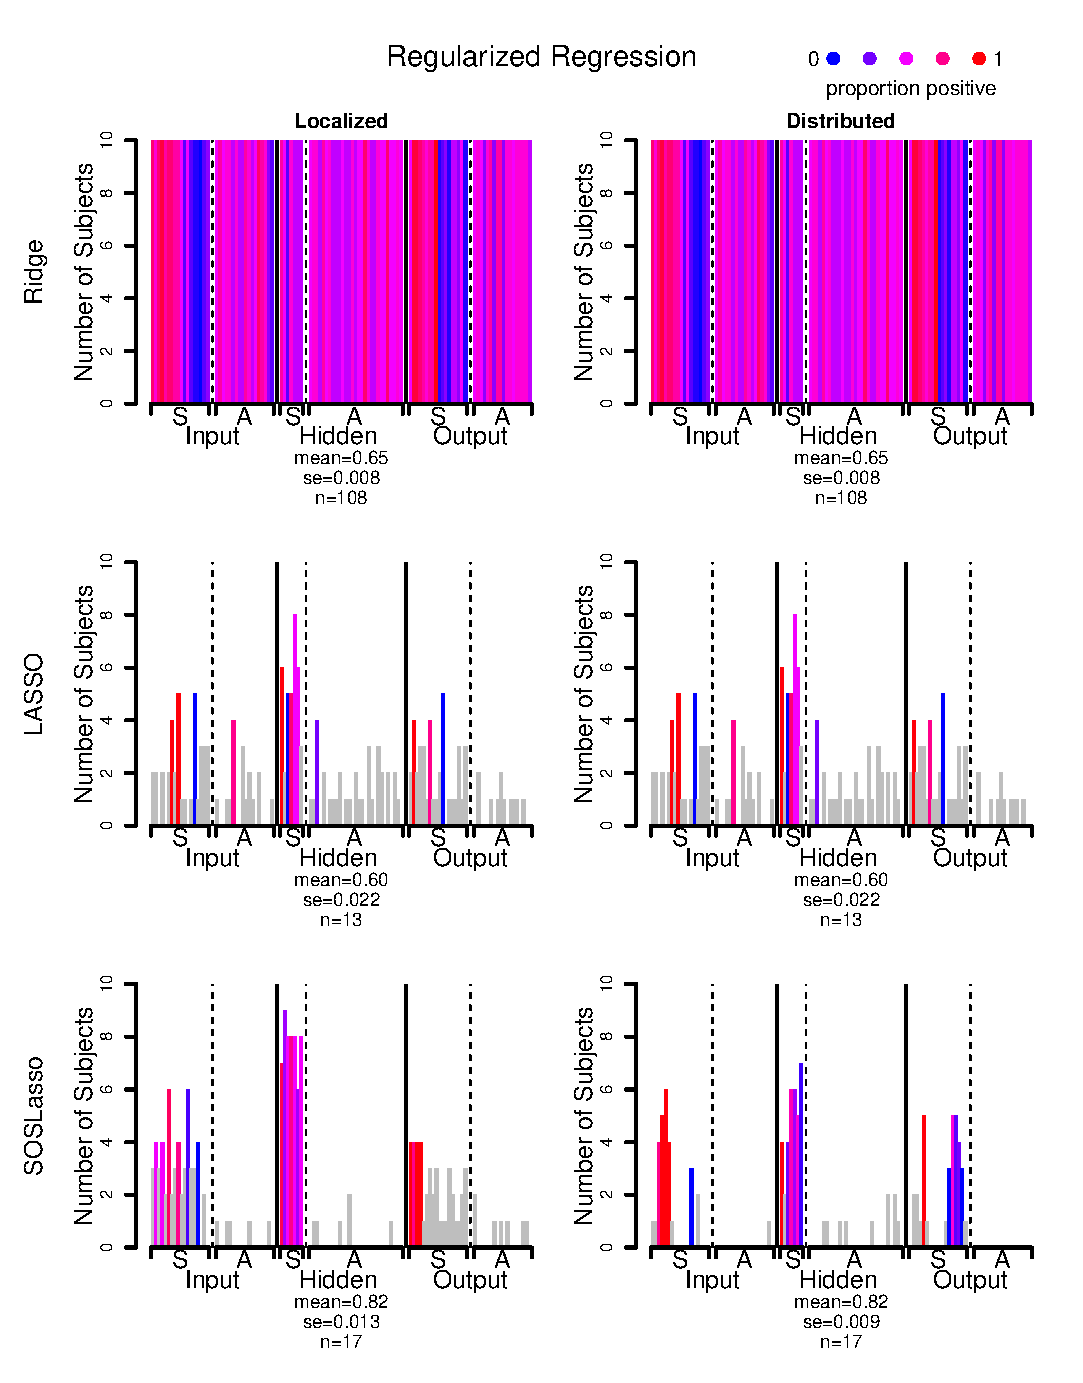
\includegraphics[width=0.75\textwidth]{figures/regression.eps}
\caption{\label{fig.regression} The results from the three regularized regression analyses. Because the model weights themselves are biased estimates and on an arbitrary scale, the height of each bar corresponds to the number of number of times each unit was selected over subjects. Colored bars were selected more times than would be expected given the overall rate of unit selection. The blueness or redness of the bar conveys the proportion of the time each unit was assigned a positive weight over subjects. Positive weights mean that activation at that unit will push the model towards labeling the current item as belonging to domain A.}
\end{figure}

\textbf{---Figure 7 about here---}
\begin{figure}
\centering

\includegraphics[width=0.5\textwidth]{figures/cmu_searchlight.eps}
\caption{\label{fig.cmu_searchlight} Information map yielded from applying searchlight to the Mitchell et al (2003) ``star-plus'' dataset, for one slice of the brain. The redness at each point indexes the number of times a searchlight centered on that voxel yielded above chance classification over subjects.}
\end{figure}

\textbf{---Figure 8 about here---}
\begin{figure}
\centering
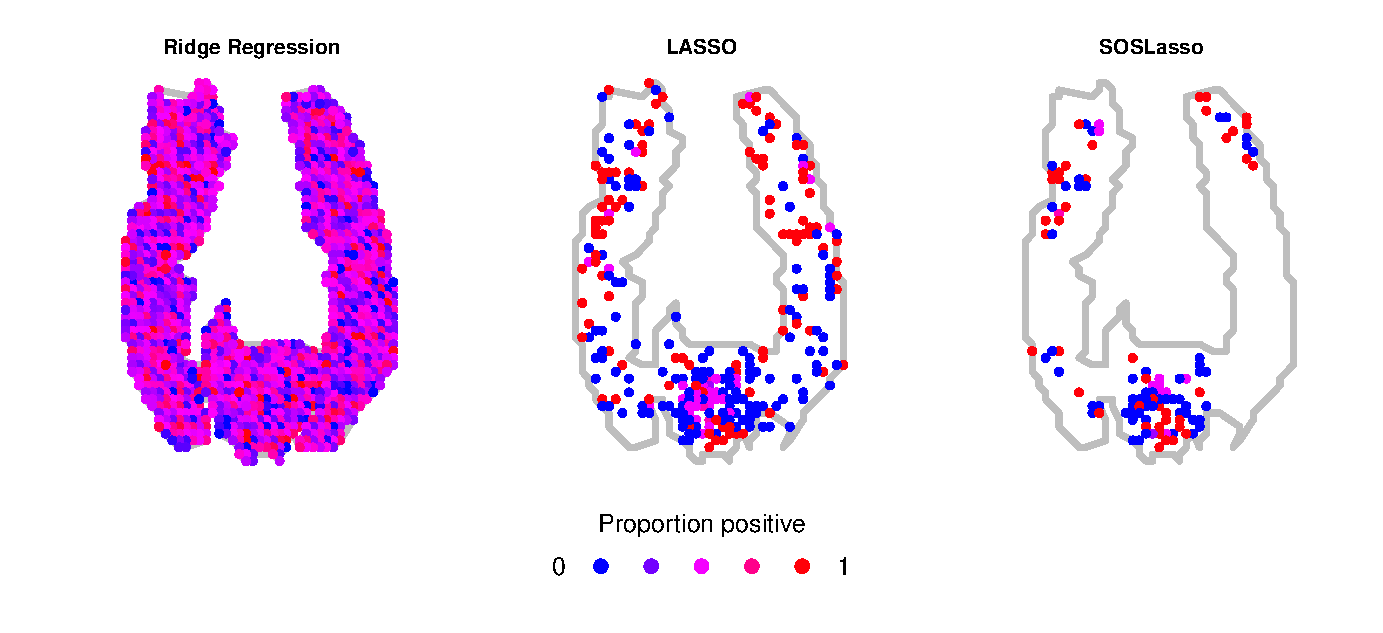
\includegraphics[width=.9\textwidth]{figures/cmu_regression.eps}
\caption{\label{fig.cmu_regression}  The information maps yielded from applying the three regularized regression analyses to the same ``star-plus'' dataset. Because the solutions are very sparse for LASSO and SOSLasso, all voxels selected for any subject are plotted. The blueness or redness of the dots conveys the proportion of the time each unit was assigned a positive weight over subjects. Positive weights mean that activation at that unit will push the model towards labeling the current item as belonging to domain A.}
\end{figure}


\section{Discussion}
The simulations presented above consider how different methods cope with the challenges of discovering distributed representations in simplified data where the truth is known regarding which units (or rather, sets of units) distinguish between two domains. This demonstrated the interesting strengths and weaknesses of each method. The degree to which signal is localized matters, as does how similar it is across subjects. Univariate method, of course, is unable to identify the systematic hidden units. Searchlight has limitations. Ridge regression is uninterpretable. Lasso is aggressively sparse and idiosyncratic. SOSLasso balances sparsity and consistency.

Several labs have been experimenting with whole brain sparse techniques for analyzing fMRI datasets. While some of this work has found its way into more mainstream neuroscience, a great deal of this work is being published in machine learning and data mining journals. A small subset of these has 


% KEY CITATIONS
% - Jarrod and Brad, 2012
% - The MVPA 2008 winners?
% - Large-scale brain networks in cognition (Bressler & Menon, 2010)


\bibliography{/Users/lcnllab/Documents/MASTERBIB/zotero}

\end{document}
